\begin{frame}{Über JUnit}
	\begin{columns}[c]
		\begin{column}{5cm}
			\def\firstcircle{(0:1cm) circle (15mm)}
			\def\secondcircle{(-120:1cm) circle (15mm)}
			\def\thirdcircle{(120:1cm) circle (15mm)}
			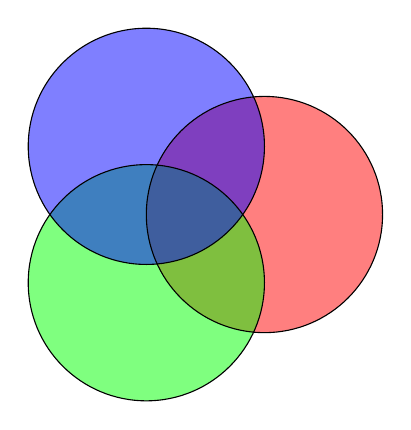
\begin{tikzpicture}
			    \begin{scope}[fill opacity=0.5]
				\fill[red] \firstcircle;
				\fill[green] \secondcircle;
				\fill[blue] \thirdcircle;
				\draw \firstcircle;
				\draw \secondcircle;
				\draw \thirdcircle;
			    \end{scope}
			\end{tikzpicture}
		\end{column}
		\begin{column}{5cm}
			\begin{block}{Kent Beck:}
				A programmer-oriented testing framework for Java.
			\end{block}
			\begin{block}{David Saff:}
				JUnit is the intersection of all possible useful Java test frameworks, not their union.
			\end{block}
			\vskip+1em
			Nicht nur für Unit Tests!
		\end{column}
	\end{columns}
\end{frame}

\begin{frame}{Warum ein Vortrag über JUnit?}
	\begin{itemize}[<+->]
		\item Jeder kennt JUnit.
		\item Wirklich?
		\item Jeder meint, JUnit zu kennen.
		\item Ich meinte es auch.
		\item Seit Version 4.0 hat sich einiges getan!
	\end{itemize}
\end{frame}

\begin{frame}{Neue Features seit Version 4.0}
\begin{center}
\begin{tikzpicture}[scale=0.9,transform shape]
  \path[every concept/.append style={font=\Large},level 1 concept/.append style={sibling angle=90,level distance=50mm},mindmap,concept color=gray,text=white]
    node[concept] {JUnit 4.8.2}
    child[grow=155,concept color=green!80]  { node[concept] {Matchers} }
    child[grow=205,concept color=blue!80]   { node[concept] {Theories} }
    child[grow=25,concept color=red!80]     { node[concept] {Rules} }
    child[grow=-25,concept color=orange!80] { node[concept] {Categories} };
\end{tikzpicture}
\end{center}
\end{frame}



{
\date{René Magritte, Untitled}
\usebackgroundtemplate{
\includegraphics[width=\paperwidth,height=\paperheight]{img/matchers/part.jpg}}
\part{Matchers}
}

\begin{frame}[fragile]{Neue Assertion: \texttt{assertThat(\dots)}}
    \begin{itemize}
        \item Neue \texttt{Assert}-Methoden:
    \begin{lstlisting}
<T> void assertThat(T actual, Matcher<T> matcher)
<T> void assertThat(String reason, T actual, Matcher<T> matcher)
\end{lstlisting}
        \item Parameter:
        \begin{description}[matcher]
            \item[reason]  Zusätzliche Beschreibung für den Fehlerfall (optional)
            \item[actual]  Tatsächlicher Wert
            \item[matcher] Hamcrest-Matcher überprüft tatsächlichen Wert
        \end{description}
    \end{itemize}
\end{frame}

\begin{frame}[fragile]{Bessere Lesbarkeit}
    \only<1>{\javainputlisting[firstline=6]{hamcrest}{BetterReadability}}
    \only<2|handout:0>{\javainputlisting[firstline=6,emph={withoutMatchers,assertEquals}]{hamcrest}{BetterReadability}}
    \only<3|handout:0>{\javainputlisting[firstline=6,emph={withMatchers,assertThat}]{hamcrest}{BetterReadability}}
    \only<4|handout:0>{\javainputlisting[firstline=6,emph={is}]{hamcrest}{BetterReadability}}
    \begin{itemize}
        \item Reihenfolge stimmt
        \item Häufig besser lesbar als herkömmliche Assertions
    \end{itemize}
\end{frame}

\begin{frame}[fragile]{Matcher kombinieren}
        Matcher lassen sich einfach kombinieren:
	    \javainputlisting[firstline=20,lastline=21,tabsize=1]{hamcrest}{WithMatchers}
\end{frame}

\begin{frame}[fragile]{Aussagekräftige Fehlermeldungen}
    \begin{block}{Herkömmliche Zusicherung ohne Beschreibung}
\javainputlisting[firstline=10,lastline=10,tabsize=1]{hamcrest}{WithoutMatchers}
Ergebnis:
\begin{lstlisting}
AssertionError: at de.andrena.junit...
\end{lstlisting}
    \end{block}	
\pause
    \begin{block}{Neue Zusicherung mit Matcher}
\javainputlisting[firstline=16,lastline=16,tabsize=1]{hamcrest}{WithMatchers}
Ergebnis:
\begin{lstlisting}
AssertionError:
Expected: not a collection containing <2>
     got: <[1, 2, 3]>
\end{lstlisting}
    \end{block}
\end{frame}

\begin{frame}{Vordefinierte Matcher}
    \begin{itemize}
        \item Vielzahl vordefinierter Matcher:
        \begin{description}[Collections]
            \item[Core] \texttt{is}, \texttt{not}, \texttt{allOf}, \texttt{anyOf}, \texttt{nullValue}, \dots
            \item[Strings] \texttt{containsString}, \texttt{startsWith}, \texttt{endsWith}, \dots
            \item[Collections] \texttt{hasItem}, \texttt{hasItems}, \texttt{isIn}, \texttt{empty}, \texttt{hasSize}, \dots
        \end{description}
        \item Bei JUnit ist nur ein kleiner Teil mit dabei:
        \begin{itemize}
            \item org.hamcrest.CoreMatchers
            \item org.junit.matchers.JUnitMatchers
        \end{itemize}
        \item Hamcrest bietet weitere Matcher (\texttt{hamcrest-all.jar}).
        \item<alert@2> Darüber hinaus lassen sich eigene Matcher definieren.
    \end{itemize}
\end{frame}

\begin{frame}{Ein eigener Matcher}{Implementierung}
	\only<1>{\javainputlisting[firstline=9]{hamcrest}{IsEmptyCollection}}
	\only<2|handout:0>{\javainputlisting[firstline=9,emph={@Override,TypeSafeMatcher,matchesSafely,describeTo}]{hamcrest}{IsEmptyCollection}}
	\only<3|handout:0>{\javainputlisting[firstline=9,emph={@Factory, empty}]{hamcrest}{IsEmptyCollection}}
\end{frame}

\begin{frame}{Ein eigener Matcher}{Benutzung}
	\javainputlisting[firstline=9]{hamcrest}{CollectionMatchersTest}
\end{frame}

\begin{frame}{Viele Matcher -- Viele Klassen}
	\begin{block}{Problem}
		\begin{itemize}
			\item Vielzahl von Klassen mit zu importierenden statischen Methoden
			\item Manuelle Konfiguration der IDE notwendig
			\item \dots bei allen Entwicklern
		\end{itemize}
	\end{block}
	\begin{block}{Lösung}
		Generierung einer eigenen Matcher-Bibliothek
	\end{block}
\end{frame}

\begin{frame}[fragile]{Generierung einer Matcher-Bibliothek}
	\begin{enumerate}
		\item Konfiguration in XML
			\lstinputlisting[language=XML,firstline=2]{java/EffectiveJUnit/src/de/andrena/junit/hamcrest/matchers.xml}
		\item Aufruf von \texttt{org.hamcrest.generator.config.XmlConfigurator}
		\item Alle mit \texttt{@Factory} annotierten Methoden werden in einer generierten Klasse zusammengefasst:
			\javainputlisting[firstline=7]{hamcrest}{Matchers}
	\end{enumerate}
\end{frame}

\begin{frame}[fragile]{Fazit: Matchers}
	\begin{itemize}
		\item Assertions lassen sich oft eleganter formulieren
		\item Manchmal sind die alten Assertion-Methoden klarer
	\end{itemize}
	\begin{block}{Problem}
		Javas Typsystem macht einem oft einen Strich durch die Rechnung
		\begin{itemize}
			\item Boxing notwendig bei primitiven Typen \begin{lstlisting}
assertThat(1 + 1, is(2))
\end{lstlisting}
			\item Mangelnde Typinferenz \begin{lstlisting}
assertThat(new TreeSet<String>(), Matchers.<String>empty());
\end{lstlisting}
		\end{itemize}
	\end{block}
\end{frame}

{
\date{Wassily Kandinsky, Composition VIII}
\usebackgroundtemplate{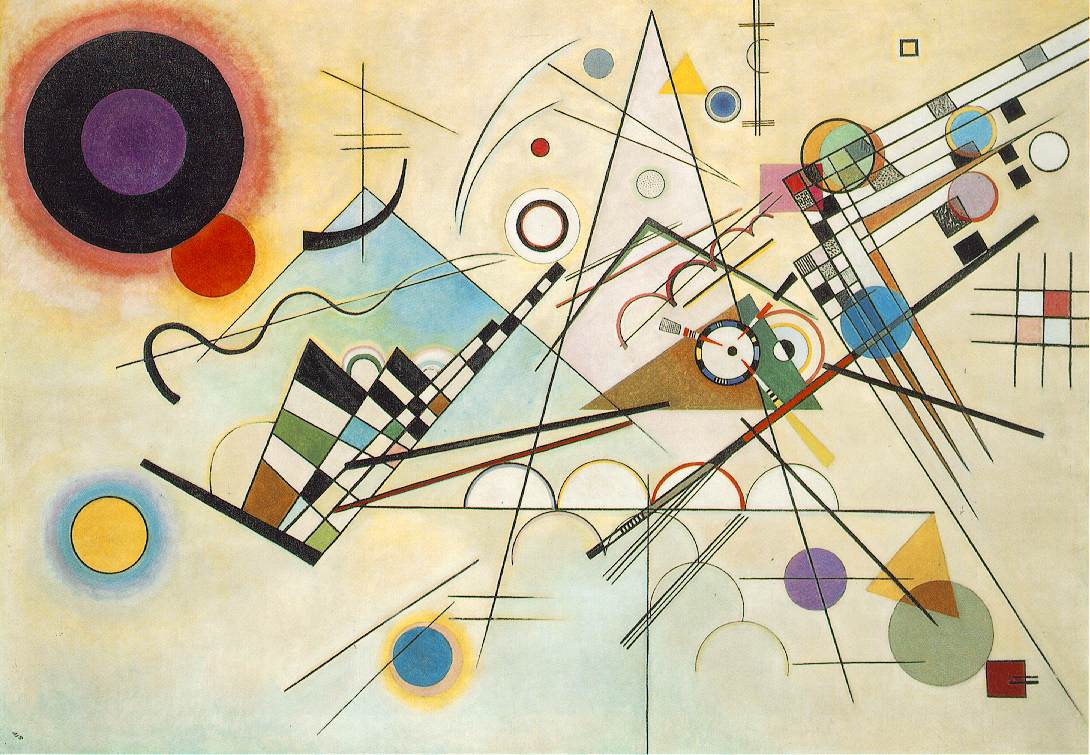
\includegraphics[width=\paperwidth,height=\paperheight]{img/theories/part.jpg}}
\part{Theories}
}

\begin{frame}[fragile]{Parametrisierte Tests}
	\begin{itemize}
		\item Seit JUnit 4.0 gibt es den \texttt{Parameterized} Test Runner.
		\item Ermöglicht Parametrisierung von Testklassen über Konstruktor
		\item Argumente werden in einer statischen Methode angegeben:
			\begin{itemize}
				\item \texttt{@Parameters}-Annotation
				\item Rückgabetyp: \verb|List<Object[]>|
			\end{itemize}
		\item Für jedes Paar von Testmethode und Argument wird eine Instanz der Testklasse angelegt und die Testmethode ausgeführt.
		\item Nützlich, wenn Berechnung mit vielen Eingabeparametern getestet werden soll.
	\end{itemize}
\end{frame}

\begin{frame}{Parametrisierte Tests}{Beispiel: Fibonacci-Zahlen}
	\only<1>{\javainputlisting[firstline=11]{fibonacci}{FibonacciParameterizedTest}}
	\only<2|handout:0>{\javainputlisting[firstline=11,emph={input, expected}]{fibonacci}{FibonacciParameterizedTest}}
	\only<3|handout:0>{\javainputlisting[firstline=11,emph={@Parameters,data}]{fibonacci}{FibonacciParameterizedTest}}
\end{frame}

\begin{frame}{Theories}
	\begin{itemize}
		\item Neu seit Version 4.4
		\item Parametrisierte Testmethode mit Vorbedingungen (Assumptions)
			\begin{itemize}
				\item \texttt{assumeThat()}
				\item \texttt{assumeTrue()}
				\item \texttt{assumeNotNull()}
			\end{itemize}
		\item \texttt{@Theory} statt \texttt{@Test}
		\item Input für Testmethoden über \texttt{@DataPoint}(\texttt{s})-Annotation
	\end{itemize}
\end{frame}

\begin{frame}{Theories}{Beispiel: Fibonacci-Zahlen}
	\only<1>{\javainputlisting[firstline=9]{fibonacci}{FibonacciTheories}}
	\only<2|handout:0>{\javainputlisting[firstline=9,emph={@Theory}]{fibonacci}{FibonacciTheories}}
	\only<3|handout:0>{\javainputlisting[firstline=9,emph={n}]{fibonacci}{FibonacciTheories}}
	\only<4|handout:0>{\javainputlisting[firstline=9,emph={assumeTrue}]{fibonacci}{FibonacciTheories}}
	\only<5|handout:0>{\javainputlisting[firstline=9,emph={@DataPoints,VALUES}]{fibonacci}{FibonacciTheories}}
	\only<6|handout:0>{\javainputlisting[firstline=9,emph={seeds}]{fibonacci}{FibonacciTheories}}
	\only<7|handout:0>{\javainputlisting[firstline=9,emph={recurrence}]{fibonacci}{FibonacciTheories}}
\end{frame}

\begin{frame}{Theories}{Beispiel: Verschiedene \texttt{@DataPoints}}
	\only<1>{\javainputlisting[firstline=9]{theories}{DifferentDataPoints}}
	\only<2|handout:0>{\javainputlisting[firstline=9,emph={@DataPoints,NUMBERS}]{theories}{DifferentDataPoints}}
	\only<3|handout:0>{\javainputlisting[firstline=9,emph={@DataPoint,A,B}]{theories}{DifferentDataPoints}}
	\only<4|handout:0>{\javainputlisting[firstline=9,emph={int,number,NUMBERS}]{theories}{DifferentDataPoints}}
	\only<5|handout:0>{\javainputlisting[firstline=9,emph={String,string,A,B}]{theories}{DifferentDataPoints}}
\end{frame}

\begin{frame}{Parameterized Tests vs. Theories}
	\begin{itemize}
		\item Definition von \texttt{@DataPoints} ist flexibler
			\begin{itemize}
				\item Konstanten oder Methoden
				\item Beliebig viele
				\item Verschiedene Typen
			\end{itemize}
		\item Parametrisierung der Test\emph{methoden}
			\begin{itemize}
				\item Kein Boilerplate-Code (Konstruktor + Instanzvariablen)
				\item Verschiedene Parametertypen möglich
			\end{itemize}
		\item \texttt{Theories} können alles, was \texttt{Parameterized} auch kann, aber mehr!
	\end{itemize}
\end{frame}

\begin{frame}{Herkömmliche Tests vs. Theories}
	\begin{itemize}
		\item Herkömmliche Tests benutzen Beispiele:
			\begin{itemize}
				\item Überprüfung des Verhaltens unter ausgewählten Eingaben
				\item Beispiele sind (hoffentlich) charakteristisch
			\end{itemize}
		\item Eine Theory verallgemeinert eine Menge von Tests:
			\begin{itemize}
				\item Vorbedingung wird explizit angegeben
				\item Sollte für alle Eingaben gelten, die Vorbedingungen erfüllen
			\end{itemize}
		\item Eingabewerte können explizit angegeben werden oder automatisch erzeugt werden
	\end{itemize}
\end{frame}


{
\date{René Magritte, Golconda}
\usebackgroundtemplate{
\includegraphics[width=\paperwidth,height=\paperheight]{img/rules/part.jpg}}
\part{Rules}
}

\begin{frame}<1-2>[label=ruledef]{Was ist eine Rule?}
	Erweiterungsmechanismus für Ablauf der Testmethoden
	\begin{block}{Beispiele:}
		\begin{itemize}
			\item<alert@2> Ausführung eigenen Codes vor bzw. nach jeder Testmethode
			\item<alert@3>  Behandlung fehlgeschlagener Tests
			\item Überprüfung zusätzlicher Kriterien nach einem Tests
			\item \dots
		\end{itemize}
	\end{block}
\end{frame}

\begin{frame}{Beispiel: TemporaryFolder}{Ohne Benutzung einer Rule}
	\only<1>{\javainputlisting[firstline=9,lastline=27]{rules}{TemporaryFolderWithoutRule}}
	\only<2|handout:0>{\javainputlisting[firstline=9,lastline=27,emph={@Before,@After,folder}]{rules}{TemporaryFolderWithoutRule}}
\end{frame}

\begin{frame}{Beispiel: TemporaryFolder}{Unter Verwendung einer Rule}
	\only<1>{\javainputlisting[firstline=9]{rules}{TemporaryFolderWithRule}}
	\only<2|handout:0>{\javainputlisting[firstline=9,emph={@Rule,folder}]{rules}{TemporaryFolderWithRule}}
\end{frame}

\againframe<3>{ruledef}

\begin{frame}{Beispiel: ExpectedException}{Ohne Benutzung einer Rule}
	\only<1>{\javainputlisting[firstline=7]{rules}{ExpectedExceptionWithoutRule}}
	\only<2|handout:0>{\javainputlisting[firstline=7,emph={expected}]{rules}{ExpectedExceptionWithoutRule}}
\end{frame}

\begin{frame}{Beispiel: ExpectedException}{Unter Verwendung einer Rule}
	\only<1>{\javainputlisting[firstline=7]{rules}{ExpectedExceptionWithRule}}
	\only<2|handout:0>{\javainputlisting[firstline=7,emph={@Rule,thrown}]{rules}{ExpectedExceptionWithRule}}
\end{frame}

\begin{frame}{Weitere vordefinierte Rules}
	\begin{block}{ErrorCollector}
		Sammelt fehlgeschlagene Assertions innerhalb einer Testmethode und gibt am Ende eine Liste der Fehlschläge aus.
	\end{block}
	\begin{block}{TestName}
		Merkt sich Namen der aktuell ausgeführten Testmethode und stellt ihn auf Anfrage zur Verfügung.
	\end{block}
	\begin{block}{Timeout}
		Wendet gleichen Timeout auf alle Testmethoden einer Klasse an.
	\end{block}
\end{frame}

\begin{frame}{Schreib deine eigenen Regeln!}
	\includegraphics<1|handout:0>[width=\textwidth]{img/rules/basisKlassen.jpg}
	\includegraphics<2>[width=\textwidth]{img/rules/basisKlassenMitTemporaryFolder.jpg}
\end{frame}

\begin{frame}{Eine eigene Regel}{Implementierung}
	\only<1>{\javainputlisting[firstline=5]{rules}{SystemProperty}}
	\only<2|handout:0>{\javainputlisting[firstline=5,emph={@Override,before,after,ExternalResource}]{rules}{SystemProperty}}
\end{frame}

\begin{frame}{Eine eigene Regel}{Benutzung}
	\only<1>{\javainputlisting[firstline=8]{rules}{SomeTestUsingSystemProperty}}
	\only<2|handout:0>{\javainputlisting[firstline=8,emph={@Rule,systemProperty}]{rules}{SomeTestUsingSystemProperty}}
\end{frame}

\begin{frame}{Vorteile von Regeln}
	\begin{block}{Wiederverwendbarkeit}
		Ermöglichen häufig benötigten Code auszulagern.
	\end{block}
	\begin{block}{Kombinierbarkeit}
		Beliebig viele Regeln in einem Test verwendbar
	\end{block}
	\begin{block}{Delegation statt Vererbung}
		Helfen Testklassenhierarchien zu vermeiden!
	\end{block}
	\begin{block}{Erweiterbarkeit}
		Eigene Regeln schreiben ist einfach.
	\end{block}
\end{frame}

{
\date{Piet Mondrian, Composition with Gray and Light Brown}
\usebackgroundtemplate{
\includegraphics[width=\paperwidth]{img/categories/part.jpg}}
\part{Categories}
}

\begin{frame}{Tests in Kategorien einteilen}
	\begin{itemize}
		\item Kategorie ist Klasse oder Interface:
			\javainputlisting[firstline=3]{categories}{Slow}
		\item Einzelner Test:
			\javainputlisting[firstline=13,lastline=15,tabsize=1]{categories}{A}
		\item Alle Tests einer Klasse:
			\javainputlisting[firstline=6]{categories}{B}
	\end{itemize}
\end{frame}

\begin{frame}{Tests in bestimmten Kategorien ausführen}
	\begin{itemize}
		\item Herkömmliche Test-Suite:
			\javainputlisting[firstline=7]{categories}{AllTests}
		\item Alle Tests in der Kategorie \texttt{Slow}:
			\javainputlisting[firstline=7]{categories}{AllSlowTests}
		\item Alle anderen Tests:
			\javainputlisting[firstline=7]{categories}{AllFastTests}
	\end{itemize}
\end{frame}

{
\date{Quint Buchholz, Mann auf einer Leiter}
\usebackgroundtemplate{
\includegraphics[width=\paperwidth,height=\paperheight]{img/summary/part.jpg}}
\part{Ausblick}
}

\begin{frame}{Was jetzt?}
	\begin{itemize}
		\item Aktualisierung auf neue Version ist einfach
		\item Alte Tests funktionieren weiterhin
		\item Neue Tests profitieren von neuen Features
		\item Alte Tests können nach und nach vereinfacht werden
		\item<alert@2> Ausprobieren!
	\end{itemize}
\end{frame}

\begin{frame}{Ausprobieren!}

	{%\Large
	\url{http://www.junit.org/}\par}\vskip+1em

	\begin{beamercolorbox}[sep=1em]{blockbackground} 
		Grau is alle Theorie – entscheidend is auf'm Platz\\
		\raggedleft -- Adi Preissler\hskip+1em\hbox{}
	\end{beamercolorbox}\vskip+1.5em
	

	{\centering\Huge
	Vielen Dank!\par}\vskip+3em

        \begin{description}[Twitter]
		\item[Mail]    \href{mailto:marc@andrena.de}{\texttt{marc@andrena.de}}
		\item[Twitter] \href{http://twitter.com/marcphilipp}{\texttt{marcphilipp}}
		\item[Blog]    \url{http://marcphilipp.tumblr.com/}
        \end{description}
\end{frame}

